%****************************************************************************************************************************************
% File: mpm4cps-ontology.tex
%
% This file is automatically generated. Please do not edit!
%****************************************************************************************************************************************
\section{Ontology Overview}

\todoAuthors{Provide ``rdfs:comment'' annotation in ontology}

Figure \ref{fig:mpm_ontology_overview} shows an overview of the MPM4CPS ontology. The details of each concept are
provided in the following subsections.

\begin{figure}[!htb]
\centering
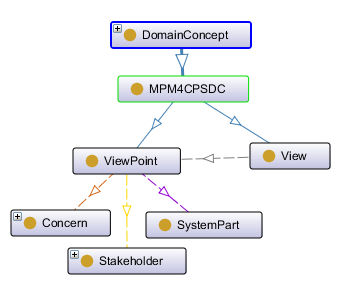
\includegraphics[width=0.5\textwidth]{figures/mpm4cps_overview.png}
\caption{Overview of the MPM4CPS ontology}
\label{fig:mpm4cps_ontology_overview}
\end{figure}



\section{Domain Concepts}

This ontology of multi-paradigm modeling contains concepts divided into sub-domains as presented in the following subsections.

\subsection{MPM4CPSDC}
\label{subsecDC:MPM4CPSDC}

\todoAuthors{Provide ``rdfs:comment'' annotation in ontology}

\subsubsection{View}
\label{subsubsecC:View}
\didx{View}

\todoAuthors{Provide ``rdfs:comment'' annotation in ontology}

\textbf{Subclass of}
\begin{itemize}
	\item \textbf{MPM4CPSDC} (see section \ref{subsecDC:MPM4CPSDC})
	\item \textbf{View} (see section \ref{subsubsecC:View})
\end{itemize}






\subsubsection{ViewPoint}
\label{subsubsecC:ViewPoint}
\didx{ViewPoint}

\todoAuthors{Provide ``rdfs:comment'' annotation in ontology}

\textbf{Subclass of}
\begin{itemize}
	\item \textbf{MPM4CPSDC} (see section \ref{subsecDC:MPM4CPSDC})
	\item \textbf{ConcernedElement} (see section \ref{subsubsecC:ConcernedElement})
	\item \textbf{ViewPoint} (see section \ref{subsubsecC:ViewPoint})
	\item \textbf{ViewPoint} (see section \ref{subsubsecC:ViewPoint})
\end{itemize}

\section{Properties}


\subsection{hasStakeholders}
\label{subsecP:hasStakeholders}
\todoAuthors{Provide ``rdfs:comment'' annotation in ontology}
Subproperty of:
None


Domains:
\begin{itemize}
	\item \textbf{ViewPoint} (see section \ref{subsubsecC:ViewPoint})
\end{itemize}


Ranges:
\begin{itemize}
	\item \textbf{Stakeholder} (see section \ref{subsubsecC:Stakeholder})
\end{itemize}




\subsection{hasSystemPart}
\label{subsecP:hasSystemPart}
\todoAuthors{Provide ``rdfs:comment'' annotation in ontology}
Subproperty of:
None


Domains:
\begin{itemize}
	\item \textbf{ViewPoint} (see section \ref{subsubsecC:ViewPoint})
\end{itemize}


Ranges:
\begin{itemize}
	\item \textbf{SystemPart} (see section \ref{subsubsecC:SystemPart})
\end{itemize}




\subsection{hasViewpoint}
\label{subsecP:hasViewpoint}
\todoAuthors{Provide ``rdfs:comment'' annotation in ontology}
Subproperty of:
None


Domains:
\begin{itemize}
	\item \textbf{View} (see section \ref{subsubsecC:View})
\end{itemize}


Ranges:
\begin{itemize}
	\item \textbf{ViewPoint} (see section \ref{subsubsecC:ViewPoint})
\end{itemize}




\subsection{isCharacterizedBy}
\label{subsecP:isCharacterizedBy}
\todoAuthors{Provide ``rdfs:comment'' annotation in ontology}
Subproperty of:
None


Domains:
\begin{itemize}
	\item \textbf{ViewPoint} (see section \ref{subsubsecC:ViewPoint})
\end{itemize}


Ranges:
\begin{itemize}
	\item \textbf{Concern} (see section \ref{subsubsecC:Concern})
\end{itemize}




\subsection{isSupportedBy}
\label{subsecP:isSupportedBy}
\todoAuthors{Provide ``rdfs:comment'' annotation in ontology}
Subproperty of:
None


Domains:
\begin{itemize}
	\item \textbf{ViewPoint} (see section \ref{subsubsecC:ViewPoint})
\end{itemize}


Ranges:
\begin{itemize}
	\item \textbf{Formalism} (see section \ref{subsubsecC:Formalism})
\end{itemize}




